\chapter{Many-body dispersion method}\label{chap:mbd}

{\sffamily This chapter presents new developments within the many-body dispersion (MBD) method, namely the reciprocal-space formulation, the MBD dielectric constant, several analytical results for the MBD wave function, and the analysis of the MBD nuclear forces and self-consistency.
Some of these results are used in the following chapters.
All the presented results have been implemented in program `pymbd' \citep{HermannZ17}, which is a standalone Python program as well as a Fortran library included in electronic-structure programs FHI-aims and DFTB+.
}

\section{Reciprocal-space formulation}

In a crystal, the matrices involved in the multipole expansion of the polarizability are infinite, and the normal real-space formalism becomes intractable.
The most straightforward resolution is to cut a sufficiently large piece of the crystal consisting of multiple unit cells, a supercell, and apply periodic boundary conditions by summing the dipole operator over the periodic images.
As shown below, this formalism, while conceptually simple, is not very efficient.
The supercell approach is an unnecessary complication that introduces the issue of slow convergence with respect to the supercell size and makes the MBD calculation computationally as expensive as the corresponding KS-DFT calculation in some cases.
The formalism developed in this section resolves these problems.

A more natural formulation uses the discrete version of the Fourier transformation in~\eqref{eq:fourier-discrete}.
The trace over the infinite number of atoms in a crystal in the MBD version of the ACFD formula in~\eqref{eq:mbd-rpa} is then transformed into a trace over atoms in a single unit cell and the reciprocal-space vectors from the first Brillouin zone, $\mathbf q$,
\begin{gather}
\begin{aligned}
  E_\text{c,lr}^\text{MBD}
    &=\frac1{2\pi}\int_0^\infty\mathrm du
    \operatorname{Tr}_{\mathbf qp\mathbb R^3}\big(
      \ln(1+\boldsymbol\alpha_\text{eff}(\mathrm iu)\mathbf T_\text{lr}(\mathbf q))
    \!\big) \\
  &=\frac{(2\pi)^3}{\Omega_\text{UC}}\int\mathrm d\mathbf q\sum_{n=1}^{3N}\frac{\tilde\omega_n(\mathbf q)}2-\sum_{p=1}^N3\frac{\omega_p}2
\end{aligned} \\
\boldsymbol\alpha_{\text{eff},p}(\mathbf q,\mathrm iu)=\sum_{\mathbf R}\boldsymbol\alpha_{\text{eff},\mathbf R_p,\mathbf R+\mathbf R_p}(\mathrm iu)\mathrm e^{\mathrm i\mathbf q\cdot\mathbf R}=\boldsymbol\alpha_{\text{eff},p}(\mathrm iu) \\
\mathbf T_{\text{lr},pq}(\mathbf q)=\sum_{\mathbf R}\mathbf T_{\text{lr},\mathbf R_p,\mathbf R+\mathbf R_q}\mathrm e^{-\mathrm i\mathbf q\cdot(\mathbf R_p-\mathbf R-\mathbf R_q)}
\end{gather}
The diagonalization of $\mathbf Q(\mathbf q)$ that leads to $\tilde{\boldsymbol\omega}(\mathbf q)$ maps again exactly on the solution of the Fourier-transformed dipole-coupled Hamiltonian, and the diagonalizing vectors, $\mathbf V(\mathbf q)$, correspond to periodic collective electron oscillations with wavelength $2\pi/|\mathbf q|$, described by collective coupled coordinates $\boldsymbol\xi'(\mathbf q)$.
\citet{BuckoJPCM16} presented the reciprocal-space formulation of MBD without performing the analytic integration over the frequency.

\begin{figure}
\makebox[\textwidth][c]{
\begin{tikzpicture}
\node[below right, anchor=base] at (0,0) {{\bfseries a}};
\node[below right] at (-.5,.5) {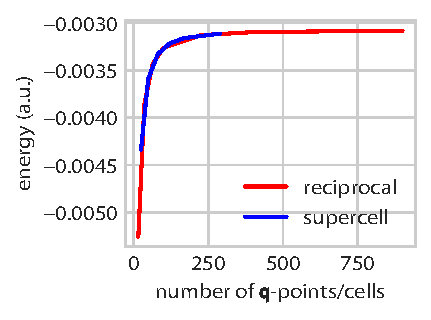
\includegraphics{media/convergence-graphene.pdf}};
\node[below right, anchor=base] at (\linewidth/2,0) {{\bfseries b}};
\node[below right] at (\linewidth/2-.5,.5) {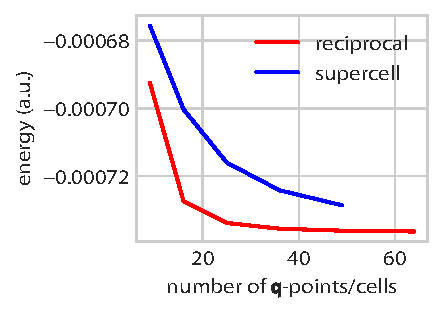
\includegraphics{media/convergence-argon.pdf}};
\end{tikzpicture}
}
\caption{\textbf{Convergence of energy in the supercell and reciprocal-space approach.}
Different convergence behavior for the 2D graphene layer (\textbf a) and the 3D argon crystal (\textbf b).
}\label{fig:mbd-convergence}
\end{figure}

The reciprocal-space formulation provides superior computational efficiency compared to the supercell approach for two reasons.
The only two computationally demanding tasks in calculating the MBD energy are the formation of the dipole operator, with complexity $O(N^2)$, $N$ being the number of atoms, and the diagonalization or inversion of matrices, with complexity $O(N^3)$.
Except for the smallest systems, the latter dominates.
The reciprocal-space integration over $\mathbf q$ is easily performed on an equidistant grid of $N_q$ vectors, and the calculation of the MBD energy then involves $N_q$ diagonalizations of the matrix $\mathbf Q(\mathbf q_n)$.
Each diagonalization has a computational complexity $O(N^3)$, $N$ being the number of atoms in the unit cell, and the total complexity is $O(N_q N^3)$.
In effective 1D and 2D systems (chains and layers), the rates of convergence of the energy with respect to the number of cells in the supercell, $N_\text c$, and to the number of points in the $\mathbf q$-grid are equal (Figure~\ref{fig:mbd-convergence}a), so for a given desired accuracy, $N_\text c=N_q$.
But the computational cost of the supercell calculation is $O\big((N_\text cN)^3\big)=O\big(N_\text c^3N^3)$, $N_\text c^2$ times larger than that of the reciprocal-space calculation.
The second reason for the better efficiency of the reciprocal-space formulation is that because the lattice sums of the dipole operator are not absolutely convergent in 3D systems, the energy converges slower with $N_\text{c}$ in the supercell approach than with $N_q$ in the reciprocal-space formulation for 3D systems (Figure~\ref{fig:mbd-convergence}b), so for a given required accuracy, $N_q<N_\text c$.

The lattice sum in the definition of $\mathbf T_\text{lr}(\mathbf q)$ can be efficiently computed using the Ewald summation in~\eqref{eq:ewald}.
The optimum balance between the computational cost of the real-space and reciprocal-space sum in the Ewald sum is reached by setting $\alpha=2.5/\sqrt[3]{\Omega_\text{UC}}$ (a.u.).
Using the real-space cutoff of $6/\alpha$ and reciprocal-space cutoff of $10\alpha$ then leads to MBD energies that are accurate up to 10 significant digits with respect to fully converged references, while the computational cost is typically by two or more orders of magnitude smaller compared to sufficiently converged calculations of MBD energies without Ewald summation.

\section{Dielectric function from MBD}

All approximate vdW methods based on the range-separated ACFD formula can be tested in two independent ways.
Testing against accurate reference polarizabilities gives information about $\boldsymbol\alpha_\text{eff}$ and $\mathbf T_\text{eff}$, but is independent of the range-separation mechanism expressed in $\mathbf T_\text{lr}$, whereas comparison against benchmark interaction energies tests all these three components combined.
For bulk material, there is no straightforward measurable equivalent of the total polarizability of a molecule.
(The total polarizability of a finite crystal sample depends on its shape.)
But an indirect measure of the bulk polarizability is provided by the macroscopic dielectric function.

Using the definitions in Section~\ref{sec:dielectric} and the Fourier transformation, $\mathcal F$, of the gradient operator, the dielectric function of the MBD model can be calculated straightforwardly,
\begin{gather}
\begin{aligned}
  \hat{\mathbf q}\cdot\boldsymbol\epsilon_\text{M}(u)\hat{\mathbf q}&=\lim_{\mathbf q\rightarrow0}\frac1{1+v(|\mathbf q|)\chi_{\mathbf 0\mathbf 0}(\mathbf q,u)} \\
  &=\lim_{\mathbf q\rightarrow0}\frac1{1+\frac{4\pi}{|\mathbf q|^2}\mathcal F[\boldsymbol\nabla\cdot\boldsymbol\nabla'\cdot\boldsymbol\alpha]_{\mathbf 0\mathbf 0}(\mathbf q,u)} \\
  &=\lim_{\mathbf q\rightarrow0}\frac1{1+\frac{4\pi}{|\mathbf q|^2}\mathbf q\cdot\boldsymbol\alpha_{\mathbf 0\mathbf 0}(\mathbf q,u)\mathbf q} \\
  &=\lim_{\mathbf q\rightarrow0}\frac1{1+4\pi\hat{\mathbf q}\cdot\boldsymbol\alpha_{\mathbf 0\mathbf 0}(\mathbf q,u)\hat{\mathbf q}} \\
  &\approx\lim_{\mathbf q\rightarrow0}\frac1{1+\frac{4\pi}{\Omega_\text{UC}}\hat{\mathbf q}\cdot\big(\sum_{pq}\boldsymbol\alpha_{pq}(\mathbf q,u)\!\big)\hat{\mathbf q}} \\
\end{aligned} \\
\boldsymbol\alpha(\mathbf q,u)=\big(\boldsymbol\alpha_\text{eff}^{-1}(u)+\mathbf T_\text{eff}(\mathbf q,u)\!\big)^{-1}
\end{gather}
The Unsöld approximation inherent in the MBD polarizability makes this approach of little use for the dynamic dielectric function, but the static dielectric constant should be represented as accurately as total polarizabilities of molecules.
Here, the use of the Ewald summation is crucial, since the required cutoff of the full real-space summation diverges as $\mathbf q\rightarrow0$.

In a simple cubic lattice, the bare dipole operator, $\mathbf T(\mathbf q)$, can be written in closed form for small $\mathbf q$,
\begin{equation}
  \mathbf T(\mathbf q)=\frac{4\pi}{\Omega_{\text{UC}}}(\hat{\mathbf k}\otimes\hat{\mathbf k}-\tfrac13\mathbf I)+O(|\mathbf q|)
\end{equation}
The expression for the dielectric function above then yields the Clausius--Mossotti equation,
\begin{equation}
  \frac{\epsilon_\text{M}(0)-1}{\epsilon_\text{M}(0)+2}=\frac{4\pi}3\frac{\alpha_\text{eff}(0)}{\Omega_\text{UC}}
\end{equation}
With more complex unit cells and the effective dipole operator from MBD, the resulting dielectric function is in general anisotropic.
Therefore, this approach can be interpreted as a generalization of the Clausius--Mossotti approximation.

\section{Properties of dipole-coupled wave function}

The diagonalization of the $\mathbf Q$ matrix of the MBD Hamiltonian in~\eqref{eq:dosc-hamil} results in the coupled resonance frequencies, $\tilde{\boldsymbol\omega}$, which give the MBD energy, as well as the eigenvectors, $\mathbf V=(\mathbf v_1\mathbf v_2\ldots)$, which define the coupled coordinates, $\hat{\boldsymbol\xi}=\mathbf V^\mathrm T\boldsymbol\xi$, in which the MBD Hamiltonian decouples into a noninteracting Hamiltonian.
The ground-state wave function is the product of harmonic-oscillator ground-state wave functions,
\begin{equation}
\psi_0(\{\tilde\xi_n\})=\prod_n\left(\frac{\tilde\omega_n}{\pi}\right)^\frac14\exp\left(-\tfrac12\tilde\omega_n\tilde\xi_n^2\right)
\label{eq:mbd-wave}
\end{equation}
This section presents several new analytical results for this correlated wave function, some of which are used in Chapter~\ref{chap:pi-pi}.

\subsection{Charge density}

When interpreted as an approximation to the full electronic Hamiltonian, the pseudo electrons in the MBD Hamiltonian effectively model the polarizable electrons in the valence shells of atoms.
One may then ask what is the charge density of these pseudo electrons, how is it different from the noninteracting system, and whether this change captures the true electron-density redistribution caused by long-range electron correlation.

The charge density of any system of $N$ charged particles is defined as an expectation value of the charge-density operator,
\begin{equation}
n(\mathbf r)=\langle\Psi|\sum_i q_i|\mathbf r_i=\mathbf r\rangle\langle\mathbf r_i=\mathbf r|\Psi\rangle=\idotsint\mathrm d\mathbf r_1\cdots\mathrm d\mathbf r_N\sum_i q_i\delta(\mathbf r-\mathbf r_i)\Psi(\{\mathbf r_j\})^2
\label{eq:density}
\end{equation}
To evaluate this expression for~\eqref{eq:mbd-wave}, we first transform the wave function back to $\boldsymbol\xi$ and gather the product of the exponentials,
\begin{equation}
\Psi(\{\xi_i\})=\left(\prod_i\left(\frac{\tilde\omega_i}{\pi}\right)^\frac14\right)\exp\Bigg(-\tfrac12\sum_{jk}\underbrace{\sum_i V_{ji}\tilde\omega_i V_{ki}}_{\Omega_{jk}}\xi_j\xi_k\Bigg)
\label{eq:wavefnc}
\end{equation}
In the following, we use $\sum_{i\notin A}$ for a sum that skips the $A$-th particle and $\sum_{i\in A}$ for a sum over the three Cartesian coordinates of the $A$-th particle.
For a given $A$, we divide the sum over $jk$ according to the order of $\xi_{i\in A}$,
\begin{equation}
\begin{aligned}
\sum_{jk}\Omega_{jk}\xi_j\xi_k&=\sum_{\substack{j\notin A\\k\notin A}}\Omega_{jk}\xi_j\xi_k+2\sum_{\substack{p\in A\\k\notin A}}\Omega_{pk}\xi_p\xi_k+2\sum_{\substack{p\in A\\q\in A}}\Omega_{pq}\xi_p\xi_q \\
&\equiv\boldsymbol\xi'^{\mathrm T}_A\boldsymbol\Omega''_A\boldsymbol\xi'_A+2\boldsymbol\xi_A'^{\mathrm T}\boldsymbol\Omega'_A\boldsymbol\xi_A+\boldsymbol\xi_A^{\mathrm T}\boldsymbol\Omega_A\boldsymbol\xi_A
\end{aligned}
\end{equation}
The linear term can be removed by completing the square with respect to $\boldsymbol\xi'_A$,
\begin{equation}
\sum_{jk}\Omega_{jk}\xi_j\xi_k=({\boldsymbol\xi'}^{\mathrm T}_A-\mathbf h_A^{\mathrm T})\boldsymbol\Omega''_A(\boldsymbol\xi'_A-\mathbf h_A)+\boldsymbol\xi_A^{\mathrm T}\boldsymbol\Omega_A\boldsymbol\xi_A-\boldsymbol\xi_A^{\mathrm T}\boldsymbol\Omega'^{\mathrm T}_A\boldsymbol\Omega_A''^{-1}\boldsymbol\Omega_A'\boldsymbol\xi_A
\label{eq:completesq}
\end{equation}
Here, $\mathbf h_A$ is some quantity that does not depend on $\boldsymbol\xi'_A$.
We can now factor out the exponential and the $3N$-dimensional integral,
\begin{equation}
n(\mathbf r)=\sum_A q_A\left(\idotsint\mathrm d\mathbf r_1\cdots\mathrm d\mathbf r_{A-1}\mathrm d\mathbf r_{A+1}\mathrm d\cdots\mathbf r_N\right)\int\mathrm d\mathbf r_A\delta(\mathbf r-\mathbf r_A)\ldots
\end{equation}

First, we evaluate the integrals in parentheses.
Because $\mathbf h_A$ is just a constant coordinate shift, and the integrals are over the whole space, $\mathbf h_A$ can be transformed away.
Furthermore, we can rotate $\boldsymbol\Omega''_A$ into a new basis where it becomes diagonal, which factors the $3(N-1)$-dimensional integral into a product of $3(N-1)$ 1-dimensional integrals over Gaussian functions of the form $\exp(-\bar\omega_{A,i}\bar\xi_{A,i}^2)$, where $\bar\omega_{A,i}$ are the eigenvalues of $\boldsymbol\Omega''_A$.
(The factor of $\frac12$ disappears due to the square of the wave function.)

Second, the integral over $\mathbf r_A$ picks the value of the following function at point $\mathbf r$ via the $\delta$-function,
\begin{equation}
\exp\big(-\boldsymbol\xi_A^\mathrm T(\underbrace{\boldsymbol\Omega_A-{\boldsymbol\Omega'}^\mathrm T_A\boldsymbol\Omega_A''^{-1}\boldsymbol\Omega_A'}_{\boldsymbol\Omega^{(A)}})\boldsymbol\xi_A\big)
\end{equation}
Combining~\eqref{eq:density},~\eqref{eq:wavefnc},~\eqref{eq:completesq}, and the previous two paragraphs, and transforming from $\boldsymbol\xi_A$ back to $\mathbf r_A$, we get
\begin{equation}
n(\mathbf r)=\sum_A q_A\left(\frac{m_A}\pi\right)^\frac32\sqrt{\frac{\prod_{i=1}^{3N}\tilde\omega_i}{\prod_{i=1}^{3(N-1)}\bar\omega_{A,i}}}\exp\big(-m_A(\mathbf r-\mathbf R_A)^\mathrm T\boldsymbol\Omega^{(A)}(\mathbf r-\mathbf R_A)\big)
\label{eq:mbd-density}
\end{equation}

\subsection{First-order perturbation correction}

The dipole-coupled wave function can serve as a zeroth-order Hamiltonian in a perturbation expansion with the perturbation equal to the difference between the full Coulomb interaction and the dipole interaction, $\hat V_{ee}-\hat V_\mathbf{pp}$.
The first-order correction does not capture any correlation energy from the higher multipoles (those start at second order), but it can serve as a measure of how effective is the Gaussian-screened dipole potential of MBD at mimicking the full Coulomb interaction at short range.

The first-order perturbation energy is just the expectation value of the perturbation Hamiltonian for the ground state,
\begin{equation}
E^{(1)}_\text{MBD}=\langle\psi_0|V_\text{ee}-V_{\mathbf{pp}}|\psi_0\rangle
\end{equation}
The expectation value of the Coulomb operator is a sum of two-particle terms,
\begin{equation}
\langle\psi_0|\tfrac12\sum_{AB}\frac{q_A q_B}{\lvert\mathbf r_A-\mathbf r_B\rvert}|\psi_0\rangle
\end{equation}
In analogy to the calculation of $n(\mathbf r)$, for each particle pair we rotate the $3(N-2)$ coordinates that are not in the Coulomb term such that the corresponding integrals become integrals over Gaussian functions, and then evaluate the remaining 6-dimensional integral over $\mathbf r_A$ and $\mathbf r_B$.

Introducing $\boldsymbol\xi_{AB}=(\boldsymbol\xi_A\boldsymbol\xi_B)$, a 6-dimensional vector, and $\boldsymbol\Omega^{(AB)}$ which is an equivalent of $\boldsymbol\Omega^{(A)}$ from the previous section, we can write the necessary integral as
\begin{equation}
I_1=\iint\mathrm d\boldsymbol\xi_A\mathrm d\boldsymbol\xi_B \frac{\exp\big(-\boldsymbol\xi_{AB}^\mathrm T\boldsymbol\Omega^{(AB)}\boldsymbol\xi_{AB}\big)}{\lvert\mathbf r_A-\mathbf r_B\rvert}
\label{eq:intcoulomb}
\end{equation}
We start by rewriting the Coulomb potential as an integral,
\begin{equation}
\frac1{\lvert\mathbf r_A-\mathbf r_B\rvert}=\frac2{\sqrt\pi}\int_0^\infty\mathrm du\exp(-\lvert\mathbf r_A-\mathbf r_B\rvert^2u^2)
\end{equation}
Inserting into $\eqref{eq:intcoulomb}$, and transforming to $\mathbf r_A$, we get a 7-dimensional integral over a Gaussian,
\begin{multline}
I_1=2\sqrt{\frac{m_A m_B}\pi}\iint\mathrm d\mathbf r_A\mathrm d\mathbf r_B\int_0^\infty\mathrm du \\
\times\exp\big[-(\mathbf r_{AB}-\mathbf R_{AB})^\mathrm T\boldsymbol\Omega_m'^{(AB)}(\mathbf r_{AB}-\mathbf R_{AB})-\mathbf r_{AB}^\mathrm T\mathbf U_2\mathbf r_{AB}\big]
\end{multline}
Here, $\boldsymbol\Omega'^{(AB)}$ absorbed the masses and $\mathbf U_2$ is defined as
\begin{equation}
\mathbf U_2=u^2\begin{pmatrix}
1&0&0&-1&0&0\\
0&1&0&0&-1&0\\
0&0&1&0&0&-1\\
-1&0&0&1&0&0\\
0&-1&0&0&1&0\\
0&0&-1&0&0&1
\end{pmatrix}
\end{equation}
Following with the integrand only, we rearrange terms and complete the square with respect to $\mathbf r_{AB}$,
\begin{multline}
\exp\big[-\mathbf r_{AB}^\mathrm T(\boldsymbol\Omega_m'^{(AB)}+\mathbf U_2)\mathbf r_{AB}+2\mathbf R_{AB}^\mathrm T\boldsymbol\Omega_m'^{(AB)}\mathbf r_{AB}-\mathbf R_{AB}^\mathrm T\boldsymbol\Omega_m'^{(AB)}\mathbf R_{AB}\big] \\
=\exp\big[-(\mathbf r_{AB}-\mathbf h_{AB})^\mathrm T(\boldsymbol\Omega_m'^{(AB)}+\mathbf U_2)(\mathbf r_{AB}-\mathbf h_{AB})\big] \\
\times\exp\big[-\mathbf R_{AB}^\mathrm T\big(\boldsymbol\Omega_m'^{(AB)}-\boldsymbol\Omega_m'^{(AB)}(\boldsymbol\Omega_m'^{(AB)}+\mathbf U_2)^{-1}\boldsymbol\Omega_m'^{(AB)}\big)\mathbf R_{AB}\big]
\end{multline}

As in the charge-density calculation, the first exponential can be shifted and rotated into a diagonal form, upon which the spatial integrals can be easily evaluated,
\begin{equation}
\iint\mathrm d\mathbf r_A\mathrm d\mathbf r_B\exp\big[-\mathbf r_{AB}^\mathrm T(\boldsymbol\Omega_m'^{(AB)}+\mathbf U_2)\mathbf r_{AB}\big]=\frac{\pi^3}{\sqrt{\prod_{i=1}^6\lambda_{AB,i}(u)}}
\end{equation}
Here, $\lambda_{AB,i}(u)$ are the eigenvalues of $(\boldsymbol\Omega_m'^{(AB)}+\mathbf U_2)$. The remaining 1-dimensional integral over $u$ from 0 to $\infty$ has a finite integrand that decays exponentially to zero, and can be quickly evaluated numerically.

Combining all parts together, we get
\begin{multline}
\langle\Psi|\tfrac12\sum_{AB}\frac{q_A q_B}{\lvert\mathbf r_A-\mathbf r_B\rvert}|\Psi\rangle
=\frac12\sum_{AB}q_A q_B\sqrt{\frac{\prod_{i=1}^{3N}\tilde\omega_i}{\prod_{i=1}^{3(N-2)}\bar\omega_{AB,i}}} \\
\times\int_0^\infty\mathrm du\frac{\exp\big[-\mathbf R_{AB}^\mathrm T\big(\boldsymbol\Omega_m'^{(AB)}-\boldsymbol\Omega_m'^{(AB)}(\boldsymbol\Omega_m'^{(AB)}+\mathbf U_2)^{-1}\boldsymbol\Omega_m'^{(AB)}\big)\mathbf R_{AB}\big]}{\sqrt{\prod_{i=1}^6\lambda_{AB,i}(u)}}
\label{eq:coulombrr}
\end{multline}

The calculation of the dipole term, $\langle\psi_0|V_\mathbf{pp}|\psi_0\rangle$, is straightforward.
First, we transform the dipole potential to the coupled basis and gather the prefactors,
\begin{equation}
  \tilde T_{ij}=\sum_{kl}C_{ki}C_{lj}\omega_k\omega_l\sqrt{\alpha_{k}(0)\alpha_{l(0)}}T_{kl}
\end{equation}
Then,
\begin{multline}
\langle\Psi|V_\mathbf{pp}|\Psi\rangle=\langle\Psi|\tfrac12\sum_{ij}\tilde\xi_i\tilde\xi_j\tilde T_{ij}|\Psi\rangle \\
=\frac12\sum_{i\neq j}\tilde T_{ij}\left(\frac{\tilde\omega_i\tilde\omega_j}{\pi^2}\right)^\frac14\int\mathrm d\tilde\xi_i\tilde\xi_i\exp\left(-\frac12\tilde\omega_i\tilde\xi_i^2\right)\int\mathrm d\tilde\xi_j\tilde\xi_j\exp\left(-\frac12\tilde\omega_j\tilde\xi_j^2\right) \\
+\frac12\sum_{i}\tilde T_{ii}\sqrt{\frac{\tilde\omega_i}{\pi}}\int\mathrm d\tilde\xi_i\tilde\xi_i^2\exp\left(-\tilde\omega_i\tilde\xi_i^2\right)=\sum_i\frac{\tilde T_{ii}}{4\tilde\omega_i}
\label{eq:dipoleterm}
\end{multline}
The $i\neq j$ terms vanished because the integrands are odd functions.

\subsection{Anisotropic Gaussian screening}

The technique used in the previous section can be also used to generalize the Gaussian screening of the Coulomb interaction, used in MBD to derive the effective dipole interaction, to anisotropic Gaussian charge densities.
This might be used to construct appropriate range separation for atomic fragments with anisotropic polarizabilities, which is investigated in Chapter~\ref{chap:polarizability}.
Integrals of the same kind are routinely evaluated in all quantum-chemistry algorithms based on Gaussian basis sets, but those are always with isotropic Gaussian functions.

The electrostatic energy of two Gaussian unit-charge densities located at $\mathbf R_A$ with anisotropic widths $\boldsymbol\sigma_A=1/\sqrt{\mathbf K_A}$ is expressed as an integral similar in form to~\eqref{eq:intcoulomb},
\begin{equation}
I_2(\mathbf K_1,\mathbf K_2)=\frac{\sqrt{\det(\mathbf K_1\mathbf K_2)}}{\pi^3}\iint\mathrm d\mathbf r_1\mathrm d\mathbf r_2\frac{\mathrm e^{-(\mathbf r_1-\mathbf R_1)\cdot\mathbf K_1(\mathbf r_1-\mathbf R_1)}\mathrm e^{-(\mathbf r_2-\mathbf R_2)\cdot\mathbf K_2(\mathbf r_2-\mathbf R_2)}}{\lvert\mathbf r_1-\mathbf r_2\rvert}
\end{equation}
The prefactor ensures proper normalization,
\begin{equation}
\lim_{a\rightarrow\infty} I_2(a\mathbf K_1,a\mathbf K_2)=\frac1{\lvert\mathbf R_1-\mathbf R_2\rvert}
\end{equation}
By identifying $m_A=1$ and $\boldsymbol\Omega^{(12)}\equiv\mathbf K=\mathbf K_1\oplus\mathbf K_2$, $I_2$ is mapped to $I_1$ of the previous section, and the final result is obtained by following the same procedure,
\begin{equation}
I_2(\mathbf K_1,\mathbf K_2)=\frac{2}{\sqrt\pi}\int_0^\infty\mathrm du\sqrt{\frac{\det\mathbf K}{\det(\mathbf K+\mathbf U_2)}}\exp\left[-\mathbf R^\mathrm T\left(\mathbf K-\mathbf K(\mathbf K+\mathbf U_2)^{-1}\mathbf K\right)\mathbf R\right]
\end{equation}
As before, the integrand is finite everywhere and decays exponentially to zero, so the integral can be efficiently evaluated by numerical quadrature.

For the isotropic case, $\mathbf K_A=\mathbf I/\sigma_A^2$, this reduces to~\eqref{eq:mayer},
\begin{equation}
\begin{aligned}
I_1(\sigma_1,\sigma_2)&=\frac2{\sqrt\pi}\int_0^\infty\mathrm du\left(1+u^2(\sigma_1^2+\sigma_2^2)\right)^{-\frac32}\exp\left[-\frac{u^2\lvert\mathbf R_1-\mathbf R_2\rvert^2}{1+u^2(\sigma_1^2+\sigma_2^2)}\right] \\
&=\frac2{\sqrt\pi}\int_0^{1/\sqrt{\sigma_1^2+\sigma_2^2}}\mathrm dv\exp\left(-v^2\lvert\mathbf R_1-\mathbf R_2\rvert^2\right) \\
&=\operatorname{erf}\left(\frac{\lvert\mathbf R_1-\mathbf R_2\rvert}{\sqrt{\sigma_1^2+\sigma_2^2}}\right)\frac1{\lvert\mathbf R_1-\mathbf R_2\rvert}
\end{aligned}
\end{equation}

The corresponding dipole operator is obtained by applying the tensor gradient,
\begin{gather}
\begin{aligned}
  \boldsymbol\nabla_{\mathbf R_1}\otimes\boldsymbol\nabla_{\mathbf R_2}I_2&\equiv
  \boldsymbol\nabla_{\mathbf R_1}\otimes\boldsymbol\nabla_{\mathbf R_2}\int_0^\infty\mathrm du i_2(u)=
  \int_0^\infty\mathrm du\boldsymbol\nabla_{\mathbf R_1}\otimes\boldsymbol\nabla_{\mathbf R_2} i_2(u) \\
  &=\int_0^\infty\mathrm du\big(-2\mathbf K_{12}+4(\mathbf K_{11}\mathbf R_1+\mathbf K_{12}\mathbf R_2)\otimes(\mathbf K_{12}\mathbf R_1+\mathbf K_{22}\mathbf R_2)\big)i_2(u)
\end{aligned} \\
  \begin{bmatrix}\mathbf K_{11}&\mathbf K_{12}\\\mathbf K_{12}&\mathbf K_{22}\end{bmatrix}\equiv\mathbf K-\mathbf K(\mathbf K+\mathbf U_2)^{-1}\mathbf K
\end{gather}

\subsection{Interaction energy decomposition}\label{sec:decom}

The interaction energy of two systems, $S_1$, $S_2$, is calculated with any total-energy method as the difference between the energy of the combined system and the subsystems,
\begin{equation}
  E^\text{(int)}(S_1,S_2)=E(S_1S_2)-E(S_1)-E(S_2)
\end{equation}
By construction, the pairwise vdW methods give a clear interpretation of the interaction energy in terms of pairs of atoms (fragments) in which the atoms are from different subsystems,
\begin{equation}
  E_\text{c,lr}^\text{(int)}(S_1,S_2)\approx-\sum_{\mathclap{A\in S_1,B\in S_2}}C_{6,{AB}}\frac{f(\mathbf R_A,\mathbf R_B)}{|\mathbf R_A-\mathbf R_B|^6}
\end{equation}
In the pairwise picture, the total collective oscillations in the system are decomposed into oscillations between individual pairs of atoms, and because this decomposition is identical in the total system and the individual subsystems, only the inter-system oscillations contribute to the interaction energy.
But in MBD, the total long-range correlation energy has the form of a sum of energies of the individual collective oscillations, which are fully delocalized and different in the total system and the subsystems.
Using the transformation between the uncoupled and coupled coordinates, however, the coupled oscillation energies of the subsystems can be projected into the coupled basis of the system and vice versa, which leads to a decomposition of the MBD interaction energy into the individual collective oscillations of the system.
This provides a clear physical picture of the binding that is utilized in Chapter~\ref{chap:pi-pi}.

The MBD interaction energy between two subsystems is expressed in terms of the coupled oscillation frequencies of the system, $\tilde{\boldsymbol\omega}$, and of the subsystems, $\tilde{\boldsymbol\omega}_1$, $\tilde{\boldsymbol\omega}_1$, and the uncoupled oscillation frequencies in the system, $\boldsymbol\omega$, and in the subsystems, $\boldsymbol\omega_1$, $\boldsymbol\omega_2$,
\begin{equation}
  E_\text{MBD}^\text{(int)}=\sum_{n=1}^{3N}\frac{(\tilde{\boldsymbol\omega})_n}2-\sum_{n'=1}^{3N}\frac{(\tilde{\boldsymbol\omega}_1\oplus\tilde{\boldsymbol\omega}_2)_{n'}}2
	-\sum_{n''=1}^{3N}\frac{({\boldsymbol\omega}-{\boldsymbol\omega}_1\oplus{\boldsymbol\omega_2})_{n''}}2
	\label{eq:mbd-int}
\end{equation}
Here, $n$ runs over the coupled coordinates of the system, $n'$ over coupled coordinates of the subsystems, and $n''$ over the uncoupled coordinates, and we wish to project the frequencies in such a way that the whole expression is a single sum either over $n$ or over $n'$.
In general, the effective noninteracting frequency of a given oscillator in the subsystem and in the total system are not equal in MBD, $\boldsymbol\omega\neq\boldsymbol\omega_1\oplus\boldsymbol\omega_2$, due to the slightly different Hirshfeld partitioning and short-range polarizability screening between the system and the subsystems.

Using the eigenvectors, $\mathbf V_1=(\mathbf v_1\mathbf v_2\ldots)$, $\mathbf V_2$, of the subsystem MBD matrices, $\mathbf Q_1$, $\mathbf Q_2$, and the eigenvectors, $\mathbf V$, of the total-system MBD matrix, $\mathbf Q$, we can construct a projector from the basis of the coupled subsystem coordinates, $\tilde{\boldsymbol\xi}_1\oplus\tilde{\boldsymbol\xi}_2$, to the basis of the coupled system coordinates, $\tilde{\boldsymbol\xi}$,
\begin{equation}
  \mathbf P=\mathbf V^\mathrm T(\mathbf V_1\oplus\mathbf V_2)
\end{equation}
This projector is orthonormal and retains the norm of a vector, but the total MBD energy is a 1-norm of the vector of oscillation energies, $E_\text{MBD}=|\boldsymbol\omega/2|_1$, which is retained by an elementwise (Hadamard) square of the projector,
\begin{equation}
  (\mathbf P^{\circ2})_{ij}=(\mathbf P)_{ij}^2
\end{equation}
Likewise, $(\mathbf V^{\circ2})^\mathrm T$ and $(\mathbf V_1^{\circ2}\oplus\mathbf V_2^{\circ2})^\mathrm T$ are projectors from the uncoupled basis of noninteracting oscillators to the coupled basis of the total system and the subsystems, respectively.
With these projectors at hand,~\eqref{eq:mbd-int} can be expressed as a single sum over the coupled coordinates of the system or the subsystems,
\begin{gather}
	E_\text{MBD}^\text{(int)}=\sum_{n=1}^{3N}\tfrac12\left(\tilde{\boldsymbol\omega}-\mathbf P^{\circ2}(\tilde{\boldsymbol\omega}_1\oplus\tilde{\boldsymbol\omega}_2)-(\mathbf V^{\circ2})^\mathrm T({\boldsymbol\omega}-{\boldsymbol\omega}_1\oplus{\boldsymbol\omega_2})\right)_n \label{eq:decom-1}\\
	E_\text{MBD}^\text{(int)}=\sum_{n'=1}^{3N}\tfrac12\left((\mathbf P^{\circ2})^\mathrm T\tilde{\boldsymbol\omega}-\tilde{\boldsymbol\omega}_1\oplus\tilde{\boldsymbol\omega}_2-(\mathbf V_1^{\circ2}+\mathbf V_2^{\circ2})^\mathrm T({\boldsymbol\omega}-{\boldsymbol\omega}_1\oplus{\boldsymbol\omega_2})\right)_{n'}\label{eq:decom-2}
\end{gather}
The vectors under the summation signs can now be interpreted as different decompositions of the MBD interaction energy into the coupled oscillations.

\section{Nuclear forces and self-consistency}

In this section, we analyze the problem of nuclear forces in a combined KS-DFT+MBD calculation.
Nuclear forces are the (negative of) total derivatives of the energy with respect to the positions of the nuclei, and are the necessary quantity for structure optimization, calculations of vibration spectra, and derived quantities.
As such, they are one of the cornerstones of computational chemistry and computational material physics.

In the following, we assume that the KS calculation is done in a finite one-electron basis, $\{|\mu\rangle\}$, which leads to the description of any particular KS state, $|\Psi\rangle$, in terms of the matrix elements, $P_{\mu\nu}$, of the density-matrix operator, $|\Psi\rangle\langle\Psi|$.
This enables expressing any measurable quantity, such as energy or the electron density, $n$, in terms of the density matrix,
\begin{equation}
\begin{aligned}
	n(\mathbf r)&=\langle\Psi|\hat n(\mathbf r)|\Psi\rangle=\langle\Psi|\sum_\mu|\mu\rangle\langle\mu|\hat n(\mathbf r)\sum_\nu|\nu\rangle\langle\nu|\Psi\rangle \\
	&=\sum_{\mu\nu}\langle\mu|\Psi\rangle\langle\Psi|\nu\rangle\langle\mu|\hat n(\mathbf r)|\nu\rangle
	=\sum_{\mu\nu}P_{\mu\nu}\varphi_\mu(\mathbf r)\varphi_\nu(\mathbf r)
\end{aligned}
\end{equation}

The total KS energy, $E_\text{KS}$, is a system-dependent (via the external potential) functional of the electron density, and hence of the density matrix and the one-electron basis.
In a standard KS calculation, the nuclear coordinates and the one-electron basis are fixed, and the KS ground state is found by minimizing the total energy (via the HK theorem) with respect to the density matrix, so that the partial derivatives are zero, $\partial E_\text{KS}/\partial P_{\mu\nu}=0$.
The total derivative of the KS energy consists of three terms via the chain rule ($\alpha=x,y,z$),
\begin{equation}
\frac{\mathrm dE_\text{KS}(\{R_{A\alpha}\},\{\varphi_\mu\},\mathbf P)}{\mathrm d R_{B\beta}}=\underbrace{\frac{\partial E_\text{KS}}{\partial R_{B\beta}}}_{\mathclap{\text{Feynman forces}}}+\underbrace{\sum_{\mu\nu}\frac{\partial E_\text{KS}}{\partial P_{\mu\nu}}\frac{\partial P_{\mu\nu}}{\partial R_{B\beta}}}_{=0}+\underbrace{\sum_\mu\int\mathrm d\mathbf r\frac{\delta E_\text{KS}}{\delta\varphi_\mu(\mathbf r)}\frac{\partial\varphi_\mu(\mathbf r)}{\partial R_{B\beta}}}_\text{Pulay forces}
\end{equation}
The first term is the explicit derivative, which is equal to the electrostatic force from the electron density on the nucleus $B$ \citep{FeynmanPR39}, the second term is zero because of the energy minimization, and the third term is nonzero only when the one-electron basis depends on the nuclear coordinates.

The MBD energy, $E_\text{MBD}$, is a function of the nuclear coordinates and of the Hirshfeld volumes (eq.~\ref{eq:hirshfeld-vol}), $V_A=\int\mathrm d\mathbf r\,n(\mathbf r)v_A(\mathbf r)$, which in turn are functionals of the electron density, and hence of the density matrix and the one-electron basis.
The total derivative is obtained via chain rules,
\begin{multline}
\frac{\mathrm dE_\text{MBD}(\{R_{A\alpha}\},\{V_A\})}{\mathrm dR_{B\beta}}=\frac{\partial E_\text{MBD}}{\partial R_{B\beta}}+\sum_A\frac{\partial E_\text{MBD}}{\partial V_A}\frac{\mathrm dV_A}{\mathrm dR_{B\beta}} \\
=\frac{\partial E_\text{MBD}}{\partial R_{B\beta}}+\sum_A\frac{\partial E_\text{MBD}}{\partial V_A}\left(\frac{\partial V_A}{\partial R_{B\beta}}+\int\mathrm d\mathbf r\frac{\delta V_A}{\delta n(\mathbf r)}\frac{\mathrm dn(\mathbf r)}{\mathrm dR_{B\beta}}\right) \\
=\frac{\partial E_\text{MBD}}{\partial R_{B\beta}}+\sum_A\frac{\partial E_\text{MBD}}{\partial V_A}\Bigg(\int\mathrm d\mathbf r\frac{\partial v_A(\mathbf r)}{\partial R_{B\beta}}n(\mathbf r)+\int\mathrm d\mathbf r\,v_A(\mathbf r)\Big(\sum_{\mu\nu}\frac{\partial n(\mathbf r)}{\partial P_{\mu\nu}}\frac{\partial P_{\mu\nu}}{\partial R_{B\beta}}+\sum_\mu\frac{\partial n(\mathbf r)}{\partial\varphi_\mu(\mathbf r)}\frac{\partial\varphi_\mu(\mathbf r)}{\partial R_{B\beta}}\Big)\!\Bigg) \\
=\frac{\partial E_\text{MBD}}{\partial R_{B\beta}}+\sum_A\frac{\partial E_\text{MBD}}{\partial V_A}\Bigg(\int\mathrm d\mathbf r\frac{\partial v_A(\mathbf r)}{\partial R_{B\beta}}n(\mathbf r)-2\int\mathrm d\mathbf r\,v_A(\mathbf r)\sum_{\mu\in B,\nu} P_{\mu\nu}\varphi_\nu(\mathbf r)\nabla_\beta\varphi_\mu(\mathbf r)\Bigg) \\
+\sum_{\mu\nu}\underbrace{\Bigg(\sum_A\frac{\partial E_\text{MBD}}{\partial V_A}\int\mathrm d\mathbf r\,v_A(\mathbf r)\varphi_\mu(\mathbf r)\varphi_\nu(\mathbf r)\!\Bigg)}_{\partial E_\text{MBD}/\partial P_{\mu\nu}}\frac{\partial P_{\mu\nu}}{\partial R_{B\beta}}
\end{multline}

Combining the KS and MBD forces together, the final expression consists of seven terms,
\begin{multline}
\frac{\mathrm d(E_\text{KS}+E_\text{MBD})}{\mathrm dR_{B\beta}}=\text{(KS Feynman forces)}+\text{(KS Pulay forces)}
+\underbrace{\frac{\partial E_\text{MBD}}{\partial R_{B\beta}}}_\text{I}\\
+\sum_A\frac{\partial E_\text{MBD}}{\partial V_A}\Bigg(\underbrace{\int\mathrm d\mathbf r\frac{\partial v_A(\mathbf r)}{\partial R_{B\beta}}n(\mathbf r)}_\text{IIa}-\underbrace{2\int\mathrm d\mathbf r\,v_A(\mathbf r)\sum_{\mu\in B,\nu} P_{\mu\nu}\varphi_\nu(\mathbf r)\nabla_\beta\varphi_\mu(\mathbf r)}_{\text{IIb}}\Bigg)\\
+\sum_{\mu\nu}\Bigg(\underbrace{\frac{\partial E_\text{KS}}{\partial P_{\mu\nu}}}_\text{IIIa}+\underbrace{\frac{\partial E_\text{MBD}}{\partial P_{\mu\nu}}}_\text{IIIb}\Bigg)\frac{\partial P_{\mu\nu}}{\partial R_{B\beta}}
\label{eq:mbd-forces}
\end{multline}
Term I is the direct force, computed with the Hirshfeld volumes fixed, and was given independently by \citet{Blood-ForsytheCS16} and \citet{BuckoJPCM16} as analytic expressions.
This is by far the dominant part of the MBD forces.
Calculation of terms IIa and IIb requires $\partial E_\text{MBD}/\partial V_A$, also given by \citet{Blood-ForsytheCS16}.
Term IIa is the force due to the dependence of the Hirshfeld-volume weight on the nuclear coordinates, and can be calculated straightforwardly from derivatives of the radial free-atom densities.
Using a plane-wave basis set, \citet{Blood-ForsytheCS16} found that the contribution of this term to the total forces is non-negligible in a test set of peptides.
Term IIb would be equal to zero in basis sets that do not depend on the nuclear coordinates (such as plane waves), and is the equivalent of the Pulay forces for the KS energy.

Terms IIIa and IIIb arise from the dependence of the density matrix on the nuclear positions.
When the MBD calculation is performed only after the KS-DFT calculation is converged (a posteriori), then IIIa is zero, and IIIb is nonzero.
On the other hand, when the MBD KS potential, $\delta E_\text{MBD}[n]/\delta n(\mathbf r)$, is calculated and included self-consistently in the KS calculation, then the total DFT+MBD energy is minimized with respect to the density matrix, and IIIa and IIIb together are zero.
The effect of self-consistency of the pairwise TS method on the resulting electron densities was investigated by \citet{FerriPRL15}.
The MBD KS potential can be calculated directly from the knowledge of $\partial E_\text{MBD}/\partial V_A$,
\begin{equation}
	v_\text{KS,MBD}(\mathbf r)=\frac{\delta E_\text{MBD}}{\delta n(\mathbf r)}=\sum_A\frac{\partial E_\text{MBD}}{\partial V_A}\frac{\delta V_A}{\delta n(\mathbf r)}=\sum_A\frac{\partial E_\text{MBD}}{\partial V_A}v_A(\mathbf r)
\end{equation}

We have implemented the evaluation of terms IIa, IIb, and of the MBD KS potential in the FHI-aims code \citep{BlumCPC09}, which uses an atom-centered basis set, to test the relative importance of the terms in~\eqref{eq:mbd-forces}.
For testing purposes, we used 10 dimers from the S22 benchmark set of small organic dimers at equilibrium geometries, and the black allotrope of phosphorus as an instance of a layered material with strong inter-layer vdW interactions.
As a benchmark, we used 5-point finite differencing to calculate the true forces.
In all cases, we found that the difference between the forces in a self-consistent and a posteriori MBD calculation, which can serve as an estimate of the magnitude of term IIIb, is below the inherent accuracy of the KS calculation.
The terms IIa and IIb were individually non-negligible, in line with the previous results, but surprisingly, the combined term fell again below the baseline accuracy in all cases.
This explains and solidifies the empirical observation that the derivatives of Hirshfeld volumes are non-negligible in a plane-wave basis, but can be neglected altogether in atom-centered basis sets in most circumstances.
